\documentclass[a4paper,12pt,twoside]{article}

%\usepackage{ucs}
\usepackage[utf8]{inputenc}
%\usepackage{babel}
%\usepackage{fontenc}
\usepackage[pdftex]{graphicx}

\usepackage[pdftex]{hyperref}

\author{Carina Norregaard}
\title{Tutorial 2a Exercise Paper}
\date{09/14/17}

\begin{document}
 
 \maketitle
 
 \begin{center}
  \texttt{norregaard.carina@gmail.com}
 \end{center}
 
 \section{Introduction}
 \label{sec:intro}
 
 This is introduction. Summary will be given in Section \ref{sec:sum}.
 
 \section{About Linux}
 \label{sec:linux}
 
 \begin{figure}[h]
    \begin{center}
     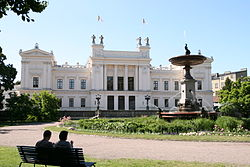
\includegraphics[width=7cm]{lunduni.jpg}
     \caption{Lund University main building}
     \label{fig:lund}
    \end{center}
 \end{figure}

 Figure \ref{fig:lund} shows a builing of \textit{Lund University}. For more details, check the Lund University Wikipedia page~\cite{lundwiki}.
 
\subsection{Linux Flavors}
\label{sec:flavors}

Table~\ref{tab:flavors} lists some Linux flavors ~\footnote{Only one is shown for simplicity}.

\begin{table}[h]
\begin{center}
 \caption{Different Flavors of Linux}
 \label{tab:flavors}
 \begin{tabular}{c|c|c|c}
  \textbf{Distribution}&RedHat&Debian&SuSE\\ \hline \hline
  Fedora 20 & X & & \\ \hline
 \end{tabular}

\end{center}
\end{table}

\section{About Mathematics}
\label{sec:math}

In-line math in \LaTeX \ is enclosed in \$ symbols. Backslash \textbackslash \ is used to denote special symbols.

Subscipts and superscripts are always math: $A_x$, $A_{xy}$, $e^x$ and $e^{x^2}$. Using underscore \_ outside math without \textbackslash \ causes big\_troubles.

All special symbols are also math: $\alpha$, $\beta$, $\gamma$, $\delta$, $\sinx$, $\hbar$, $\lambda$, $\ldots$. More information can be found in Ref.~\cite{latex}

Equation~\ref{eq:chi2} shows $\chi^2$.

\begin{equation}
\label{eq:chi2}
  \chi^2 = \sum\limits_i \left(\frac{F_i - D_i}{\sigma_i}\right)^2
\end{equation}

 
 \section{Summary}
 
 We learned the following: 
\begin{itemize}
 \item Linux is good
 \item \LaTeX \ is good for:
  \begin{enumerate}
   \item Structuring documents
   \item Writing mathematical equations
  \end{enumerate}

\end{itemize}


We can also write unformatted text using \texttt{verbatim} environment, but sometimes we have to specify this in the preamble:
\begin{verbatim}
 \usepackage{verbatim}
\end{verbatim}





 
 \begin{thebibliography}{99}
  \bibitem{lundwiki} Lund University Wikipedia page: \url{https://en.wikipedia.org/wiki/Lund_University}

  \bibitem{latex} Leslie Lamport,\textit{LaTeX: A document Preparation Sytem}, second edition, Addison-Wesley (1994).
 \end{thebibliography}

 
 \label{sec:sum}

 
 
 
\end{document}
